\graphicspath{{./chap6/images/}}  
\chapter{Admin}
\textbf{이 장은 관리자 작업과 관련된 것들을 다룬다.}

\section{공지}
서버에는 여러 학생들의 연구 및 논문 데이터가 있다. 그러므로 서버에서의 중대한 작업이 진행될 경우 사전에 공지하여 백업하도록 하는 것이 바람직하다. 리눅스 사용자 협회 오픈채팅방 등을 이용하면 된다.
\subsection{유저 관리}
adduser를 이용해 유저를 생성할 수 있다. usermod를 이용해 유저의 그룹을 관리할 수 있다. su를 이용해 사용자를 바꿀 수 있다. useradd를 사용할 경우 유저의 홈 디렉트리, bash 쉘 등이 생성되지 않으므로 adduser의 사용을 권장한다.
    \begin{lstlisting}
    $ adduser gs21000
    $ usermod -aG GROUP gs21000
    $ su gs20000
    \end{lstlisting}
\section{초기화}
서버에 중대한 문제가 발생하여 해결이 불가하거나 심히 어려운 경우 초기화가 그 해결책이 될 수 있다. 본 문서는 Ubuntu Server 20.04.2 LTS를 기반으로 작성되었다.
\subsection{설치디스크 준비}
\begin{enumerate}
    \item 2GB 이상의 USB 준비
    \item 우분투 이미지 사이트\href{https://releases.ubuntu.com/20.04/}{(링크)}에서 Ubuntu Server 20.04 준비한다. 원하는 버전을 준비하면 된다. 중요한 것은 LTS 버전을 다운로드해야 된다는 것이다. 
    \item Rufus\href{https://rufus.ie/}{(링크)} 준비
    \item Rufus 실행 후 준비한 iso 선택
    \item 준비한 USB를 선택하고 '시작' 클릭 (iso 우선 모드는 큰 상관이 없다. 
\end{enumerate}
\subsection{기타 OS 설치}
방법은 동일하다. 현재 관리자 송혁중은 OPENSUSE에 빠져 상업용 Opensuse를 무료로 사용할 수 있는 권한까지 받아 학교 서버에 설치할 수 있었지만 호환성 문제로 하지 않았다. 그러니 다른 OS는 추천하지는 않는다. 다른 OS를 깔았다가 모든 학생들이 반발하는 모습을 볼 수 있을 것이다. 특히나 데비안 계열에서 다른 계열로 변경하는 것은 비추천한다...
\subsection{Ubuntu 설치}
연구용 서버는 SRC 7층 서버실에 위치해 있다. 먼저 7층 교무실에 계시는 정덕교 선생님이나 박종화 선생님께 서버 초기화를 위해 왔음을 알여야 한다. 

테스트용서버(구서버)는 서버실에서 가장 가까운 서버렉의 제일 아래에 있다. 후면에 USB와 VGA 단자가 있고 안쪽에는 키보드, 마우스와 모니터가 있으므로 연결하여 작업하면 된다. 먼저 전원 버튼을 꾹 눌러 종료시킨 뒤 다시 눌러 시스템을 시작한다. 이후 바이오스 창이 나올 때 F2 또는 Del 키를 누르면 부팅 디스크를 선택할 수 있게 된다.
메인서버(신서버, 115.23.235.150)은 서버실의 가장 가까운 서버렉의 위에서 2번째 칸에 위치한다. gpu 10장이 들어가기 위한 것 같아보이는 서버가 신서버이다. 마찬가지지만 usb 단자가 앞면에 위치하고 있다. 
이후 설치 과정을 따라하면 된다. 이때 OpenSSH-Server를 설치하는 것을 추천한다. 또, 중간에 네트워크를 설정하는 창이 나오면 설정표\href{https://github.com/gshslinuxintro/Server-Configuration/blob/main/Network.md}{(비공개 링크)}를 보고 정덕교 선생님께 여쭤보며 작성하면 된다. 신서버를 처음 설치할때는 22.04 버전을 설치하였지만 호환성이 맞지 않는 패키지가 많았으므로 이를 해결하기 위해서 20.04로 다운그레이드를 진행하였다. 버전 업그레이드는 추천하지 않는다. (cuda의 지원 속도가 매우 느린 편)

\section{Drivers}
\textbf{이 Section은 어떤 드라이버도 깔려 있지 않은 상태에서의 설치 상황을 다룬다. 설치과정에서 자동으로 driver를 설치할 수는 있지만 추천하지 않는다.}

먼저 아래 명령어를 통해 현재 설치된 GPU에 적합한 드라이버를 찾을 수 있다.
\begin{lstlisting}
    $ ubuntu-drivers devices
\end{lstlisting}
이후 그중 하나를 골라(recommended) 설치하면 된다.
\begin{lstlisting}
    $ sudo apt install nvidia-driver-XXX (숫자)
\end{lstlisting}
적용하려면 재부팅이 필요하다.
\begin{lstlisting}
    $ sudo reboot
\end{lstlisting}
Nvidia-smi를 통해 설치를 확인할 수 있다.
\begin{lstlisting}
    $ nvidia-smi
\end{lstlisting}
\begin{figure}[H]
	\begin{center}
        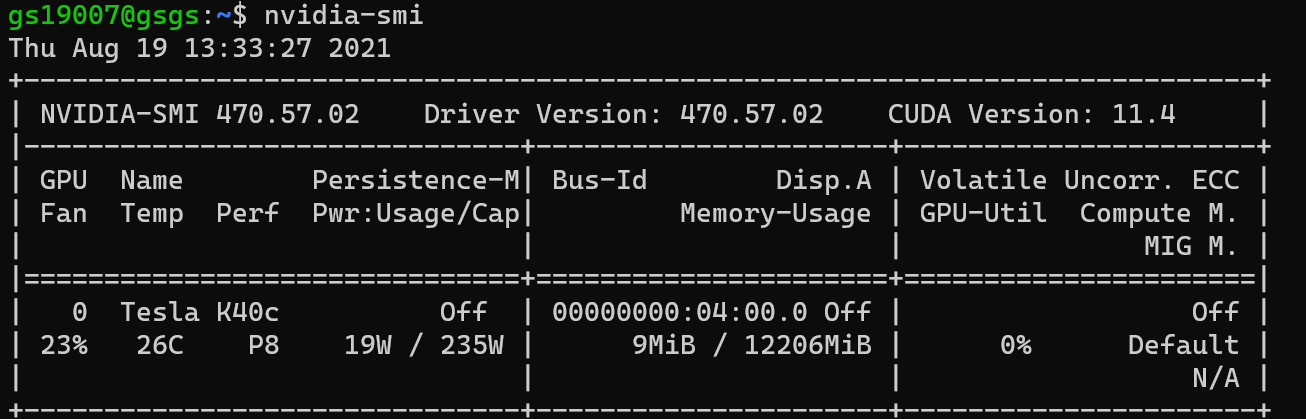
\includegraphics[width=5cm]{nvidia-smi}
        \caption{nvidia-smi}
    \end{center}
\end{figure}
여기서 CUDA Version은 권장 사항으로, 실제 CUDA 버전 및 설치 유무와는 상관 없다.


\section{CUDA 및 cuDNN}
\subsection{CUDA 설치}
기본적으로 알아야 할 사실은 CUDA가 라이브러리라는 것이다. 그렇기에 여러 CUDA 버전을 동시에 설치할 수 있다. 또, debian package로 설치하지만 않았다면 다음 명령어를 통해 쉽게 제거할 수 있음을 기억하자.
\begin{lstlisting}
    $ sudo rm -rf /usr/local/cuda*
\end{lstlisting}

CUDA 설치를 위해서는 gcc가 필요하다.
\begin{lstlisting}
    $ sudo apt-get install build-essential
\end{lstlisting}
이후 CUDA 설치를 위해 먼저 Nvidia Developer 사이트\href{https://developer.nvidia.com/cuda-toolkit-archive}{(링크)}에 들어간다.

여기서 현재 서버의 상황에 맞는 버튼들을 누른다. 참고로 CUDA 12 이후 버전들은 점진적으로 Compute Compatability가 3.x대인 GPU들에 대한 지원을 제한하고 있는데, 연구용 서버에 장착된 GPU인 Tesla K40c의 Compute Compatability는 3.5다. 따라서 11.2 이하 버전의 설치를 권장한다.
\begin{figure}[H]
	\begin{center}
        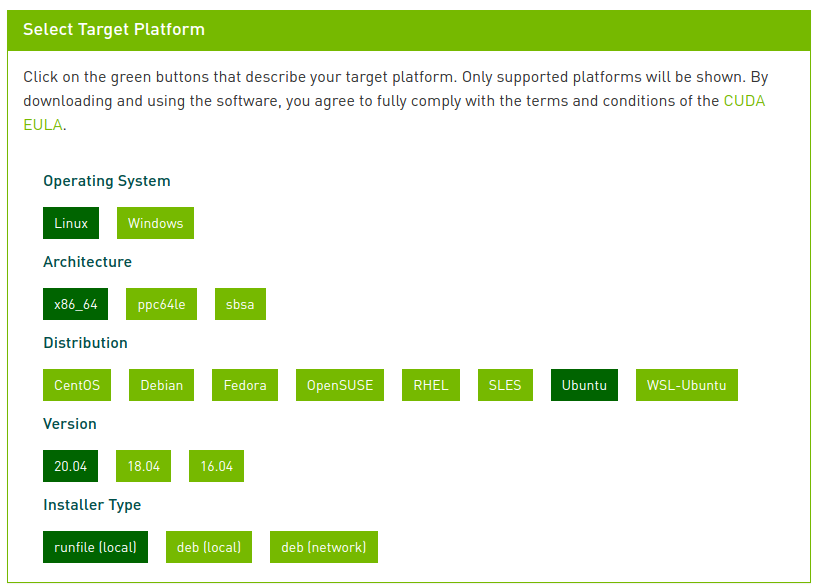
\includegraphics[width=9cm]{cuda1}
        \caption{CUDA 설치}
    \end{center}
\end{figure}
이후 지시사항에 따라 명령어를 입력하면 된다.
\begin{figure}[H]
	\begin{center}
        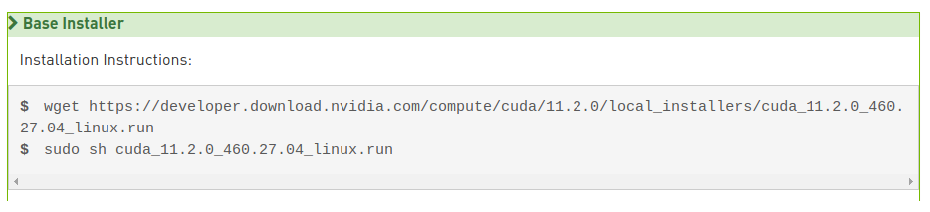
\includegraphics[width=12cm]{cuda2}
        \caption{CUDA 설치}
    \end{center}
\end{figure}


중간에 설치 프롬프트가 뜨는데, 스페이스 키를 눌러 드라이버는 설치에서 제외한다. 이후 설치를 진행하면 된다.
\begin{figure}[H]
	\begin{center}
        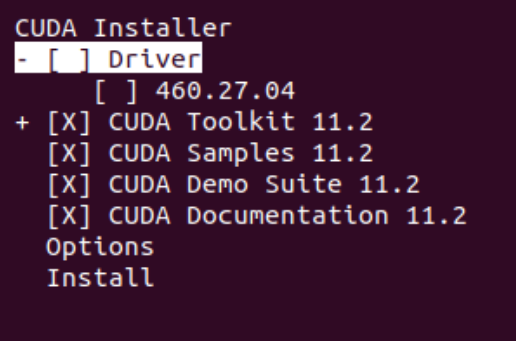
\includegraphics[width=5cm]{cuda3}
        \caption{CUDA 설치 - Drivers}
    \end{center}
\end{figure}

\subsection{환경변수 설정}
먼저 다음 명령어를 통해 CUDA를 환경변수에 등록한다. 11.2 자리에 다른 버전을 넣을 수도 있다.
\begin{lstlisting}
    $ sudo sh -c "echo 'export PATH=$PATH:/usr/local/cuda-11.2/bin' >> /etc/profile"

    $ sudo sh -c "echo 'export LD_LIBRARY_PATH=$LD_LIBRARY_PATH:/usr/local/cuda-11.2/lib64' >> /etc/profile"

    $ sudo sh -c "echo 'export CUDADIR=/usr/local/cuda-11.2' >> /etc/profile"

    $ source /etc/profile
\end{lstlisting}
이후 다음 명령어를 입력했을 때 CUDA 버전이 올바르게 출력된다면 설치 성공이다.
\begin{lstlisting}
    $ nvcc -V
\end{lstlisting}
\subsection{cuDNN 설치}
Nvidia Developer 사이트\href{https://developer.nvidia.com/cudnn}{(링크)}에 들어간다.
로그인 또는 회원가입 후 약관 및 서약에 동의하면 링크가 생긴다. 여기서 Archived cuDNN Releases에 들어가 cuDNN v8.1.1 (Feburary 26th, 2021), for CUDA 11.0,11.1 and 11.2를 다운로드 받는다.
\begin{figure}[H]
	\begin{center}
        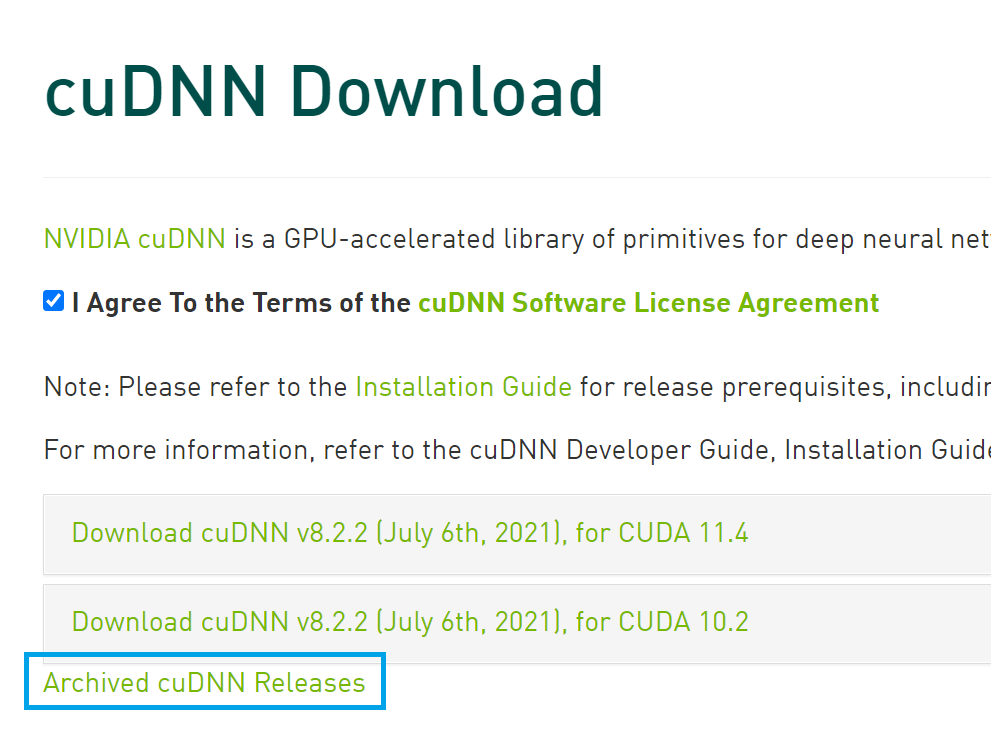
\includegraphics[width=12cm]{cudnn1}
        \caption{cuDNN 설치}
    \end{center}
\end{figure}

이 파일은 서버에서는 다운받을 수 없다. 따라서 sftp 등의 방법으로 서버에 업로드해야 한다. 이후 다음 명령어를 차례로 입력한다.
\begin{lstlisting}
    $ tar xvzf cudnn-11.2-linux-x64-v8.1.1*.tgz

    $ sudo cp cuda/include/cudnn* /usr/local/cuda/include

    $ sudo cp cuda/lib64/libcudnn* /usr/local/cuda/lib64

    $ sudo chmod a+r /usr/local/cuda/include/cudnn.h /usr/local/cuda/lib64/libcudnn*


    $ sudo ln -sf /usr/local/cuda-11.2/targets/x86_64-linux/lib/libcudnn_adv_train.so.8.1.1 /usr/local/cuda-11.2/targets/x86_64-linux/lib/libcudnn_adv_train.so.8

    $ sudo ln -sf /usr/local/cuda-11.2/targets/x86_64-linux/lib/libcudnn_ops_infer.so.8.1.1  /usr/local/cuda-11.2/targets/x86_64-linux/lib/libcudnn_ops_infer.so.8

    $ sudo ln -sf /usr/local/cuda-11.2/targets/x86_64-linux/lib/libcudnn_cnn_train.so.8.1.1  /usr/local/cuda-11.2/targets/x86_64-linux/lib/libcudnn_cnn_train.so.8

    $ sudo ln -sf /usr/local/cuda-11.2/targets/x86_64-linux/lib/libcudnn_adv_infer.so.8.1.1  /usr/local/cuda-11.2/targets/x86_64-linux/lib/libcudnn_adv_infer.so.8

    $ sudo ln -sf /usr/local/cuda-11.2/targets/x86_64-linux/lib/libcudnn_ops_train.so.8.1.1  /usr/local/cuda-11.2/targets/x86_64-linux/lib/libcudnn_ops_train.so.8

    $ sudo ln -sf /usr/local/cuda-11.2/targets/x86_64-linux/lib/libcudnn_cnn_infer.so.8.1.1 /usr/local/cuda-11.2/targets/x86_64-linux/lib/libcudnn_cnn_infer.so.8

    $ sudo ln -sf /usr/local/cuda-11.2/targets/x86_64-linux/lib/libcudnn.so.8.1.1  /usr/local/cuda-11.2/targets/x86_64-linux/lib/libcudnn.so.8

    $ sudo ldconfig
\end{lstlisting}
이후 다음 명령어를 입력했을 때 버전이 정확하게 출력되면 된다.
\begin{lstlisting}
    $ ldconfig -N -v $(sed 's/:/ /' <<< $LD_LIBRARY_PATH) 2>/dev/null | grep libcudnn
\end{lstlisting}
\section{Storage}
신서버를 구축하면서 15T짜리 디스크 레이드를 구성해야 되는 일이 생겼다. 이와 관련된 얘기들을 적을 예정. LVM groups가 무엇인가?, mount는 무엇인가?, 레이드는 무엇인가? 
